\documentclass{beamer}
\title{Le problème des dominos de Wang}
\author{Matteo Wei et Nathan Boyer}
\date{2024}
\AtBeginSection[]

\usepackage[dvipsnames]{xcolor}
\usepackage[utf8]{inputenc}
\usepackage{lmodern}
\usepackage[T1]{fontenc}
\usepackage[french]{babel}
\usepackage{bookmark}
\usepackage{graphicx}
\graphicspath{ {./images/} }
\usepackage{tikz}
\usepackage{amssymb}
\usepackage{amsmath}

\renewcommand{\le}{\leqslant}
\renewcommand{\ge}{\geqslant}
\newcommand{\R}{\mathbb R}
\newcommand{\Q}{\mathbb Q}
\newcommand{\C}{\mathbb C}
\newcommand{\N}{\mathbb N}
\newcommand{\Z}{\mathbb Z}
\newcommand{\U}{\mathbb U}
\newcommand{\id}{\mathrm{id}}
\newcommand{\ind}{\mathbbb 1}
\newcommand{\clC}{\mathrm C}
\renewcommand{\O}{\mathrm O}
\renewcommand{\o}{\mathrm o}
\newcommand{\sube}{\subseteq}
\renewcommand{\H}{\mathrel{\mathcal H}}
\newcommand{\V}{\mathrel{\mathcal V}}


\begin{document}

\frame{\titlepage}

\section{Introduction}

\begin{frame}
    \frametitle{Table des matières}
    \tableofcontents[currentsection]
  \end{frame}
  
\begin{frame}
\frametitle{Ensemble de Wang}

\begin{alertblock}{Definition}

    Un \emph{ensemble de Wang} est un triplet $(H,V,T)$ où $H$ et $V$ sont respectivement les couleurs horizontales et verticales
    et où $T \sube H^2 * V^2$ est l'ensemble des dominos. On appelera parfois aussi abusivement ensemble de Wang l'ensemble des dominos $T$.
    
\end{alertblock}

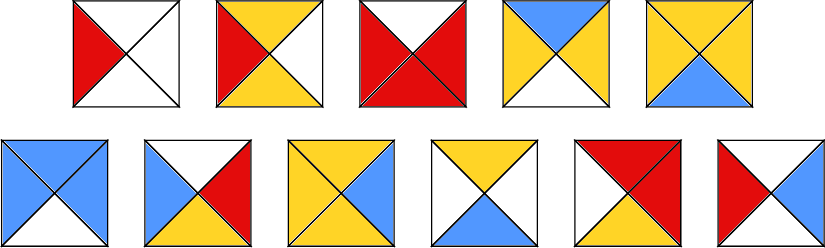
\includegraphics{ensemble_de_wang_exemple}

\end{frame}

\begin{frame}
\frametitle{Pavage}

\begin{alertblock}{Definition}

    Soit $X \sube \Z^2$ et $\tau$ un ensemble de Wang.

    Un pavage de X par $\tau$ est une fonction $f:X \to T$ avec:
    
    \[\forall (x,y) \in X, {f(x,y)}_e = {f(x+1,y)}_w \land {f(x,y)}_n = {f(x,y+1)}_s.\]
    
    Un pavage du plan par $\tau$ est un pavage de $\Z^2$.
    
\end{alertblock}

\begin{figure}

    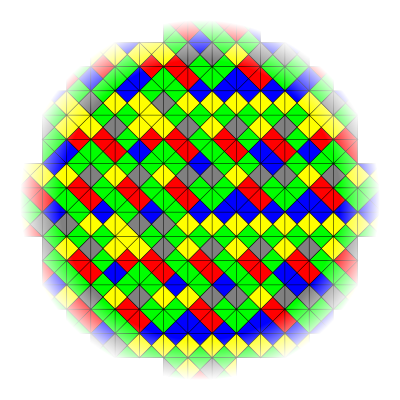
\includegraphics[scale = 0.3]{pavage_exemple}
    \centering
    
\end{figure}


\end{frame}

\begin{frame}
\frametitle{Pavage périodique et apériodique}

\begin{alertblock}{Definition}

On dit que $\tau$ est périodique s'il existe un pavage du plan périodique par $\tau$
(càd tel que $\exists (u,v) \in {\Z^*}^2, \forall (x,y) \in \Z^2, f(x,y) = f(x+u,y)=f(x,y+v)$).

On dit que $\tau$ est apériodique s'il existe au moins un pavage du plan par $\tau$ mais que tous ses pavages ne sont pas périodiques.
    
\end{alertblock}

\begin{figure}

    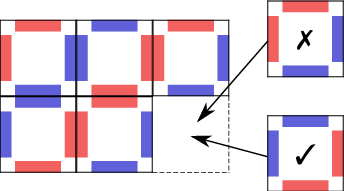
\includegraphics[scale = 0.5]{pavage_periodique}
    \centering
    
\end{figure}

\end{frame}

\begin{frame}{Conjecture de Wang}

    \begin{block}{Conjecture (Wang, 1961)}
        Un ensemble de Wang qui pave le plan est périodique.
    \end{block}
    
    \end{frame}
    
\section{Indécidabilité du problème du domino}

\subsection{Le problème du domino}

    \begin{frame}
        \frametitle{Table des matières}
        \tableofcontents[currentsection]
    \end{frame}
    
    \begin{frame}{Le problème du domino}
    
    \begin{alertblock}{Problème du domino}
        Étant donné un ensemble de Wang, est-il possible de paver le plan avec ?
    \end{alertblock}
    
    \begin{block}<2>{Proposition}
        La conjecture de Wang implique que le problème du domino est décidable.
    \end{block}
    
    \end{frame}
    
    \begin{frame}
    
    \begin{block}{Lemme (compacité)}
        Un ensemble de Wang pave le plan si, et seulement si, il pave des carrés arbitrairement grands.
    \end{block}
    
    \begin{exampleblock}<2>{Preuve de la proposition}
        Si on suppose la conjecture de Wang, alors étant donné un ensemble de Wang, il existe $n\in\N^*$ tel que:
        \begin{itemize}
            \item Soit il ne pave pas le carré $n\times n$.
            \item Soit il le pave d'une manière complétable en un pavage périodique du plan. 
        \end{itemize}
        Donc le problème du domino est décidable.
    \end{exampleblock}
    
    \end{frame}
    
    \begin{frame}{Encodage de machines de Turing par des pavages}
    
    \begin{alertblock}{Stratégie}
        Trouver une manière d'encoder une machine de Turing avec un ensemble de Wang, pour ramener le problème du domino au problème de l'arrêt.
    \end{alertblock}
    
    \begin{block}<2>{Idée}
        Représenter les états de la machine et les lettres avec des contraintes de couleur sur les bords.
    \end{block}
    
    \end{frame}
    
    \begin{frame}
        
        \begin{figure}
            \centering
            \begin{tikzpicture}[scale = 0.9]
              \foreach \x in {2, 5}
              {\fill [fill = BrickRed] (3*\x,0) rectangle (3*\x+2,2);
              \fill [fill = White] (3*\x,0) rectangle (3*\x+1/4,2);
              \fill [fill = White] (3*\x+2-1/4, 0) rectangle (3*\x+2, 2);}
              \fill [fill = Gray] (16-1/8, 1-1/8) rectangle (16+1/8, 2);
              \fill [fill = Gray] (16, 1) circle (8 pt);
              \foreach \x in {2, 3, 4, 5}
              \fill [fill = BrickRed] (3*\x,-3) rectangle (3*\x+2,-1);
              \fill [fill = Red] (6, -3) -- (7, -2) -- (8, -3) -- cycle;
              \fill [fill = Red] (9, -3) -- (10, -2) -- (11, -3) -- cycle;
              \foreach \x in {2, 3, 4, 5}
              {\fill [fill = White] (3*\x,-3) rectangle (3*\x+1/4,-1);
              \fill [fill = White] (3*\x+2-1/4, -3) rectangle (3*\x+2, -1);}
              \fill [fill = RoyalBlue] (7-1/8, -3) -- (7-1/8, -2+1/8) -- (7+1/8, -2-1/8) -- (7+1/8, -3) --cycle;
              \fill [fill = Blue] (8, -2+1/8) -- (7-1/8, -2+1/8) -- (7+1/8, -2-1/8) -- (8, -2-1/8) --cycle;
              \fill [fill = RoyalBlue] (10+1/8, -3) -- (10+1/8, -2+1/8) -- (10-1/8, -2-1/8) -- (10-1/8, -3) --cycle;
              \fill [fill = Blue] (9, -2+1/8) -- (10+1/8, -2+1/8) -- (10-1/8, -2-1/8) -- (9, -2-1/8) --cycle;
              \fill [fill = Black] (8-1/4, -3+3/2-1/8) rectangle (8, -3+3/2+1/8);
              \fill [fill = Black] (14, -3+1/2+1/8) -- (14-1/4, -3+1/2) -- (14, -3+1/2-1/8) -- cycle;
              \fill [fill = Black] (9+1/4, -3+1/2-1/8) rectangle (9, -3+1/2+1/8);
              \fill [fill = Black] (15, -3+3/2+1/8) -- (15+1/4, -3+3/2) -- (15, -3+3/2-1/8) -- cycle;
              \fill [fill = Blue] (13-1/8, -3+1-1/8) rectangle (13+1/8, -3+2);
              \fill [fill = Blue] (13-1/8, -3+1-1/8) rectangle (14, -3+1+1/8);
              \fill [fill = Blue] (13, -3+1) circle (8 pt);
              \fill [fill = Blue] (13-1/8, -3+1-1/8) rectangle (13+1/8, -3+2);
              \fill [fill = Blue] (13-1/8, -3+1-1/8) rectangle (14, -3+1+1/8);
              \fill [fill = Blue] (13, -3+1) circle (8 pt);
              \fill [fill = Blue] (16-1/8, -3+1-1/8) rectangle (16+1/8, -3+2);
              \fill [fill = Blue] (16+1/8, -3+1-1/8) rectangle (15, -3+1+1/8);
              \fill [fill = Blue] (16, -3+1) circle (8 pt);
              \foreach \x in {2, 3, 4, 5}
              \draw (3*\x,-3) rectangle (3*\x+2,-1);
              \foreach \x in {2, 5}
              \draw (3*\x,0) rectangle (3*\x+2,2);
              \node at (7, -0.5) {$\mathrm{let}(s)$};
              \node at (16, -0.5) {$\mathrm{init}(s)$};
              \node at (7, -3.5) {$\mathrm{trans}_\rightarrow(\delta_\rightarrow)$};
              \node at (13, -3.5) {$\mathrm{head}_\leftarrow(q,s)$};
              \node at (10, -3.5) {$\mathrm{trans}_\leftarrow(\delta_\leftarrow)$};
              \node at (16, -3.5) {$\mathrm{head}_\rightarrow(q,s)$};
            \end{tikzpicture}
            \label{fig:tilesidee}
          \end{figure}
    
    \end{frame}
    
    \begin{frame}
        
    \begin{alertblock}{Problèmes}
        \begin{itemize}
            \item On n'impose pas la présence d'une tête de lecture.
            \item On n'impose pas l'unicité d'une tête de lecture.
            \item On n'impose pas la présence d'un état initial.
            \item On ne contrôle pas le mot de départ.
        \end{itemize}
    \end{alertblock}
    
    \end{frame}
    
    \begin{frame}{Le problème du domino fixé}
    
    \begin{alertblock}{Définition}
        Le problème du domino fixé est celui de décider, étant donné un ensemble de Wang $T$ et un domino $t$ de l'ensemble, s'il existe un $T$-pavage de $\N^2$ avec $t$ en $(0,0)$.
    \end{alertblock}
    
    \begin{block}{Proposition (compacité)}
        C'est le cas si, et seulement si, il existe des $T$-pavages de carrés arbitrairement grands avec $t$ au coin sud-ouest. 
    \end{block}
    
    \end{frame}
    
    \begin{frame}
    
    \begin{block}{Proposition}
        Le problème du domino fixé n'est pas décidable.
    \end{block}
    
    \begin{exampleblock}<2>{Preuve}
        Étant donné une machine de Turing, on construit un ensemble de Wang qui simule les calculs de la machine sur le mot vide, et on se sert de la contrainte de domino fixé pour rajouter l'état initial.
    \end{exampleblock}
    
    \end{frame}
    
    \begin{frame}
        
        \begin{figure}
            \centering
            \begin{tikzpicture}[scale = 0.75]
              \fill [fill = Gray] (14.5-1/8, 4-1/8) rectangle (14.5+1/8, 5);
              \fill [fill = Gray] (14.5, 4) circle (8 pt);
              \fill [fill = Black] (13.5,3) rectangle (1/4+13.5,5);
              \fill [fill = Black] (13.5,3) rectangle (15.5,3+1/4);
              \fill [fill = Black] (3,3) rectangle (5,3+1/4);
              \foreach \x in {1, 2, 4}
              \fill [fill = BrickRed] (3*\x,0) rectangle (3*\x+2,2);
              \fill [fill = Red] (6, 0) -- (7, 1) -- (8, 0) -- cycle;
              \foreach \x in {1, 2, 3, 4, 5}
              \fill [fill = BrickRed] (3*\x,-3) rectangle (3*\x+2,-1);
              \fill [fill = Red] (6, -3) -- (7, -2) -- (8, -3) -- cycle;
              \fill [fill = Red] (9, -3) -- (10, -2) -- (11, -3) -- cycle;
              \foreach \x in {1, 2, 4}
              {\fill [fill = Black] (3*\x,0) rectangle (3*\x+1/4,2);
              \fill [fill = White] (3*\x+2-1/4, 0) rectangle (3*\x+2, 2);}
              \foreach \x in {1, 2, 3, 4, 5}
              {\fill [fill = White] (3*\x,-3) rectangle (3*\x+1/4,-1);
              \fill [fill = White] (3*\x+2-1/4, -3) rectangle (3*\x+2, -1);}
              \fill [fill = RoyalBlue] (7-1/8, 0) -- (7-1/8, 1+1/8) -- (7+1/8, 1-1/8) -- (7+1/8, 0) --cycle;
              \fill [fill = Blue] (8, 1+1/8) -- (7-1/8, 1+1/8) -- (7+1/8, 1-1/8) -- (8, 1-1/8) --cycle;
              \fill [fill = Blue] (13-1/8, 1-1/8) rectangle (13+1/8, 2);
              \fill [fill = Blue] (13-1/8, 1-1/8) rectangle (14, 1+1/8);
              \fill [fill = Blue] (13, 1) circle (8 pt);
              \fill [fill = Black] (8-1/4, 3/2-1/8) rectangle (8, 3/2+1/8);
              \fill [fill = Black] (14, 1/2+1/8) -- (14-1/4, 1/2) -- (14, 1/2-1/8) -- cycle;
              \fill [fill = RoyalBlue] (7-1/8, -3) -- (7-1/8, -2+1/8) -- (7+1/8, -2-1/8) -- (7+1/8, -3) --cycle;
              \fill [fill = Blue] (8, -2+1/8) -- (7-1/8, -2+1/8) -- (7+1/8, -2-1/8) -- (8, -2-1/8) --cycle;
              \fill [fill = RoyalBlue] (10+1/8, -3) -- (10+1/8, -2+1/8) -- (10-1/8, -2-1/8) -- (10-1/8, -3) --cycle;
              \fill [fill = Blue] (9, -2+1/8) -- (10+1/8, -2+1/8) -- (10-1/8, -2-1/8) -- (9, -2-1/8) --cycle;
              \fill [fill = Black] (8-1/4, -3+3/2-1/8) rectangle (8, -3+3/2+1/8);
              \fill [fill = Black] (14, -3+1/2+1/8) -- (14-1/4, -3+1/2) -- (14, -3+1/2-1/8) -- cycle;
              \fill [fill = Black] (9+1/4, -3+1/2-1/8) rectangle (9, -3+1/2+1/8);
              \fill [fill = Black] (15, -3+3/2+1/8) -- (15+1/4, -3+3/2) -- (15, -3+3/2-1/8) -- cycle;
              \fill [fill = Blue] (13-1/8, -3+1-1/8) rectangle (13+1/8, -3+2);
              \fill [fill = Blue] (13-1/8, -3+1-1/8) rectangle (14, -3+1+1/8);
              \fill [fill = Blue] (13, -3+1) circle (8 pt);
              \fill [fill = Blue] (13-1/8, -3+1-1/8) rectangle (13+1/8, -3+2);
              \fill [fill = Blue] (13-1/8, -3+1-1/8) rectangle (14, -3+1+1/8);
              \fill [fill = Blue] (13, -3+1) circle (8 pt);
              \fill [fill = Blue] (16-1/8, -3+1-1/8) rectangle (16+1/8, -3+2);
              \fill [fill = Blue] (16+1/8, -3+1-1/8) rectangle (15, -3+1+1/8);
              \fill [fill = Blue] (16, -3+1) circle (8 pt);
              \foreach \x in {1, 2, 4}
              \draw (3*\x,0) rectangle (3*\x+2,2);
              \foreach \x in {1, 4.5}
              \draw (3*\x,3) rectangle (3*\x+2,5);
              \foreach \x in {1, 2, 3, 4, 5}
              \draw (3*\x,-3) rectangle (3*\x+2,-1);
              \node at (4, 2.5) {${\mathrm{let}}^{\mathrm S}(\_)$};
              \node at (14.5, 2.5) {$\mathrm{init}$};
              \node at (4, -0.5) {${\mathrm{let}}^\mathrm W(s)$};
              \node at (7, -0.5) {$\mathrm{trans}_\rightarrow^\mathrm W(\delta_\rightarrow)$};
              \node at (13, -0.5) {$\mathrm{head}_\leftarrow^\mathrm W(q,s)$};
              \node at (4, -3.5) {${\mathrm{let}}(s)$};
              \node at (7, -3.5) {$\mathrm{trans}_\rightarrow(\delta_\rightarrow)$};
              \node at (13, -3.5) {$\mathrm{head}_\leftarrow(q,s)$};
              \node at (10, -3.5) {$\mathrm{trans}_\leftarrow(\delta_\leftarrow)$};
              \node at (16, -3.5) {$\mathrm{head}_\rightarrow(q,s)$};
            \end{tikzpicture}
            \label{fig:tiles}
          \end{figure}
    \end{frame}
    
    \begin{frame}{Vers le problème du domino}
    
    \begin{block}{Proposition}
        Le problème du domino n'est pas décidable.
    \end{block}
    
    \begin{exampleblock}<2>{Idée de la preuve}
        Construire un ensemble dont tous les pavages font apparaître des carrés vides arbitrairement grands. Le combiner avec l'ensemble de Wang de départ pour paver ces carrés avec l'ensemble de départ, en imposant la tuile sud-ouest.\\
        On déduit alors le résultat de l'indécidabilité du problème du domino fixé.
    \end{exampleblock}
    
    \end{frame}

\subsection{Complétude de problèmes de pavage}

    \begin{frame}{Complétude de problèmes de pavage}
        
    \begin{block}{Idée}
        Comme on peut facilement encoder l'exécution d'une machine de Turing avec des ensembles de Wang, il est facile d'obtenir des résultats de complétude pour des problèmes de pavage. 
    \end{block}
    
    \begin{alertblock}<2>{Définition (problèmes $\mathrm{TILING}$)}
        Soit $h:\N\to\N$ et $w:\N\to\N$ tel que $w\ge\id_\N$. Le problème de décision $\mathrm{TILING}(h,w)$, consiste, étant donné un ensemble de Wang $T$, quatre couleurs $N$, $S$, $E$ et $W$, et une suite de couleurs de longueur $n$, consiste à décider s'il existe un $T$-pavage d'un carré de taille $w(n)\times h(n)$ avec les contraintes supplémentaires que les bords nord, est et ouest soient des couleurs correspondantes et que le bord sud commence par la suite de couleurs donnée, puis continue avec la couleur $S$.\\
        On note $\mathrm{TILING}(*,w)$, le même problème, où l'on enlève les contraintes de hauteur.
    \end{alertblock}
    
    \end{frame}
    
    \begin{frame}
    
    \begin{block}{Proposition}
        Soit $k\in\N$. $\mathrm{TILING}(\exp_k,\exp_k)$ est $k\mathrm{NEXPTIME}$-complet.
      \end{block}
    
    \begin{block}{Proposition}
        Soit $k\in\N$. $\mathrm{TILING}(*,\exp_k)$ est $k\mathrm{EXPSPACE}$-complet.
    \end{block}
    
    \begin{exampleblock}<2>{Preuve}
        Dans les deux cas, on vérifie qu'un pavage est solution avec les bonnes contraintes (on a besoin de stocker qu'un seul rang).\\
        Dans l'autre sens, étant donné un problème dans la classe de complexité, on construit l'ensemble de Wang correspondant à une machine de Turing qui le décide, et on simule les calculs en imposant la suite de couleurs en entrée.
    \end{exampleblock}
    
    \end{frame}
    
    \begin{frame}
    
        \begin{figure}
            \centering
            \begin{tikzpicture}[scale = 0.6]
              \foreach \x in {1, 2, 3, 4, 5, 6}
              \fill [fill = BrickRed] (3*\x,-6) rectangle (3*\x+2,-4);
              \fill [fill = Red] (6, -6) -- (7, -5) -- (8, -6) -- cycle;
              \fill [fill = Red] (9, -6) -- (10, -5) -- (11, -6) -- cycle;
              \foreach \x in {1, 6}
              \fill [fill = BrickRed] (3*\x,-3) rectangle (3*\x+2,-1);
              \foreach \x in {1, 2, 3, 4, 5, 6}
              {\fill [fill = White] (3*\x,-6) rectangle (3*\x+1/4,-4);
              \fill [fill = White] (3*\x+2-1/4, -6) rectangle (3*\x+2, -4);}
              \fill [fill = RoyalBlue] (7-1/8, -6) -- (7-1/8, -5+1/8) -- (7+1/8, -5-1/8) -- (7+1/8, -6) --cycle;
              \fill [fill = Blue] (8, -5+1/8) -- (7-1/8, -5+1/8) -- (7+1/8, -5-1/8) -- (8, -5-1/8) --cycle;
              \fill [fill = RoyalBlue] (10+1/8, -6) -- (10+1/8, -5+1/8) -- (10-1/8, -5-1/8) -- (10-1/8, -6) --cycle;
              \fill [fill = Blue] (9, -5+1/8) -- (10+1/8, -5+1/8) -- (10-1/8, -5-1/8) -- (9, -5-1/8) --cycle;
              \fill [fill = Black] (9+1/4, -6+1/2-1/8) rectangle (9, -6+1/2+1/8);
              \fill [fill = Black] (14, -6+1/2+1/8) -- (14-1/4, -6+1/2) -- (14, -6+1/2-1/8) -- cycle;
              \fill [fill = Black] (9+1/4, -6+1/2-1/8) rectangle (9, -6+1/2+1/8);
              \fill [fill = Black] (15, -6+3/2+1/8) -- (15+1/4, -6+3/2) -- (15, -6+3/2-1/8) -- cycle;
              \fill [fill = Blue] (13-1/8, -6+1-1/8) rectangle (13+1/8, -6+2);
              \fill [fill = Blue] (13-1/8, -6+1-1/8) rectangle (14, -6+1+1/8);
              \fill [fill = Blue] (13, -6+1) circle (8 pt);
              \fill [fill = Blue] (13-1/8, -6+1-1/8) rectangle (13+1/8, -6+2);
              \fill [fill = Blue] (13-1/8, -6+1-1/8) rectangle (14, -6+1+1/8);
              \fill [fill = Blue] (13, -6+1) circle (8 pt);
              \fill [fill = Blue] (16-1/8, -6+1-1/8) rectangle (16+1/8, -6+2);
              \fill [fill = Blue] (16+1/8, -6+1-1/8) rectangle (15, -6+1+1/8);
              \fill [fill = Blue] (16, -6+1) circle (8 pt);
              \foreach \x in {1, 6}
              {\fill [fill = White] (3*\x,-3) rectangle (3*\x+1/4,-1);
              \fill [fill = White] (3*\x+2-1/4, -3) rectangle (3*\x+2, -1);
              \fill [fill = Gray] (3*\x, -1) -- (3*\x+1/4, -1-1/4) -- (3*\x+2-1/4, -1-1/4) -- (3*\x+2, -1) -- cycle;
              \draw (3*\x,-3) rectangle (3*\x+2,-1);}
              \foreach \y in {-1, -2}
              {\fill [fill = Black] (19-1/8, 3*\y) rectangle (19+1/8, 3*\y+1);
              \fill [fill = Black] (19, 3*\y+1) circle (8 pt);}
              \foreach \x in {1, 2, 3, 4, 5, 6}
              \draw (3*\x,-6) rectangle (3*\x+2,-4);
            \end{tikzpicture}
            \caption{On impose le gris comme couleur nord, le blanc pour le trois autres bords (aussi la couleur du symbole blanc)}
            \label{fig:tiles2}
          \end{figure}
    
    \end{frame}
    
    \begin{frame}
        
    \begin{block}{Corollaire}
        $\mathrm{TILING}(\id_\N,\id_\N)$ est $\mathrm{NP}$-complet, et $\mathrm{TILING}(*,\id_\N)$ est $\mathrm{PSPACE}$-complet.
    \end{block}
    
    \begin{exampleblock}<2>{Preuve}
        Cas $k=0$.
    \end{exampleblock}
    
    \end{frame}

\section{Nombre minimal de dominos pour un ensemble de Wang apériodique}

\begin{frame}
    \frametitle{Table des matières}
    \tableofcontents[currentsection]
  \end{frame}

\subsection{Définitions préalables}

\begin{frame}
\frametitle{Transducteur}

\begin{alertblock}{Definition}

Un transducteur $\tau$ est un automate qui lit une bande d'entrée bifinie et écrit sur une bande de sortie bifinie.
    
\end{alertblock}

\begin{figure}

    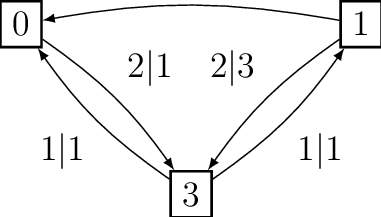
\includegraphics[scale = 1]{transducteur_exemple}
    \centering
    
\end{figure}

\begin{alertblock}{Définition}

On dit que $w \tau w'$ si $w'$ est une bande de sortie pour la bande d'entrée $w$ et le transducteur $\tau$.
    
\end{alertblock}

\end{frame}

\begin{frame}
\frametitle{Lien entre dominos et transducteurs}

On peut voir un pavage comme un transducteur.

En effet, $\forall t = (w,e,s,n) \in T$, on dit qu'il y a une transition de l'état $w$ vers l'état $e$ qui lit $n$ et écrit $s$.

Ainsi, l'ensemble de wang vu en Introduction se réécrit

\begin{center}

\begin{tikzpicture}[node distance={45mm}, main/.style = {draw, circle}] 
    \node[main] (0) {$0$};
    \node[main] (1) [right of=0] {$1$};
    \draw[->] (0) to [out=45,in=135,looseness=1] node[midway, above, pos=0.5] {$0|1$} (1);
    \draw[->] (1) to [out=-135,in=-45,looseness=1] node[midway, below, pos=0.5] {$1|0$} (0);
\end{tikzpicture} 

\end{center}

\end{frame}

\begin{frame}
\frametitle{Ensemble de Wang représenté}

\begin{figure}

    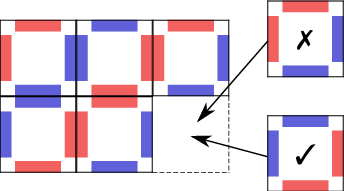
\includegraphics[scale = 0.5]{pavage_periodique}
    \centering
    
\end{figure}

\end{frame}

\begin{frame}
\frametitle{Reformulation du problème initial}

On définit également la composition de 2 transducteurs de manière naturelle.

On peut alors reformuler le problème initial de la façon suivante:

\begin{block}{Proposition}

Un ensemble de Wang admet un pavage périodique si et seulement si $\exists w \text{ mot bifini }, k \in \N, \text{ avec } w \tau^k w$.
    
\end{block}

\begin{block}{Equivalence entre 2 ensembles de Wang}

On ne s'intéresse plus aux ensembles de Wang que sous le point de vue des transducteurs.

Ainsi, 2 ensembles de Wang sont équivalents ssi leurs transducteurs définissent la même relation, càd ssi $\forall w,w', \; w \tau w' \iff w \tau' w'$.
    
\end{block}

\end{frame}

\subsection{Générer tous les ensembles de Wang de cardinal au plus 10}

\begin{frame}

\frametitle{Générer tous les ensembles de Wang de cardinal au plus 10}

Pour commencer, on va chercher à générer tous les ensembles de Wang de cardinal au plus 10 (à l'équivalence définie plus tôt près)

\begin{alertblock}{Definition}

Soit $\tau$ un ensemble de Wang. On dit que $\tau$ est minimal apériodique si $\tau$ est apériodique
et qu'aucun sous-ensemble strict de $\tau$ n'est apériodique.
    
\end{alertblock}
    
\end{frame}

\begin{frame}
\frametitle{Quelques propriétés sur les transducteurs apériodiques}

On s'intéresse ici au graphe orienté $G = (V,E)$ lié au transducteur de $\tau$.

On a alors les résultats suivants:

\begin{itemize}
    \item Soit $u,v \in V \text{ avec } uv \in E \text{ mais pas de chemin de v vers u}$, alors $\tau$ n'est pas apériodique minimal.
    \item Si $G$ a une composante fortement connexe qui est un cycle, alors $\tau$ n'est pas apériodique minimal.
    \item Si $G$ n'a qu'un sommet, alors $\tau$ n'est pas apériodique.
    \item Si $|E|-|V| \le 2$, alors $\tau$ n'est pas apériodique minimal.
\end{itemize}

\end{frame}

\begin{frame}
\frametitle{Schémas de preuve}

Pour le premier point, $(uv)$ correspond à un domino $t$ qui ne peut apparaître qu'une fois par colonne,
donc, si $\tau$ pave le plan, alors $\tau \setminus \{t \}$ aussi, d'où le résultat.

\;

Pour le deuxième point, supposons qu'il existe une telle composante. Cela veut donc dire qu'il existe $S \sube T$
tel qu'à chaque fois qu'un des dominos apparaît, la ligne entière est périodique.

Si $T$ est apériodique, on ne peut pas avoir un pavage où les dominos de $S$ apparaissent dans deux rangées différentes, car on pourrait en déduire un pavage périodique.

En conséquence, les tuiles de $S$ apparaissent dans au plus une ligne, et en utilisant le même argument que précédemment, nous déduisons que $T \setminus S$ pave le plan.


\end{frame}

\begin{frame}
\frametitle{Schémas de preuve}

    Pour le troisième point, si $G$ n'a qu'un sommet mais que $\tau$ pave le plan, alors on peut construire un pavage
    du plan tel que chaque colonne est la même.
    
    \;
    
    La preuve du dernier point est très longue (plus de $15$ pages) et ne sera donc pas détaillée ici.
\end{frame}

\begin{frame}
\frametitle{Génération de transducteurs}

On génère alors tous les transducteurs d'au plus 10 arêtes ne vérifiant aucune de ces conditions (et qui n'ont pas de sommet isolé).

On trouve alors qu'il en existe $77809$.

\end{frame}

\subsection{Tester l'apériodicité}

\begin{frame}
\frametitle{Critères d'apériodicité}

On veut maintenant tester l'apériodicité de ces différents transducteurs.

Cependant, on sait qu'un transducteur $\tau$ n'est pas apériodique si:

\begin{itemize}
    \item $\exists k \in \N$ tel que $\nexists w,w'$ avec $w \tau^k w'$ ($\tau$ ne pave pas le plan).
    \item $\exists k \in \N$ tel que $\exists w$ avec $w \tau^k w$ ($\tau$ est périodique).
\end{itemize}
    
\end{frame}

\begin{frame}
\frametitle{Algorithme pour tester l'apériodicité}

L'algorithme est alors évident: Pour chaque $k \in \N$, calculer $\tau^k$ et tester si il y a un des $2$ cas précédents,
jusqu'à ce que l'ordinateur ne dispose plus d'assez de mémoire (en effet, comme on l'a vu plus haut, ce problème est indécidable).
Dans ce cas, on doit alors étudier le cas à la main.

On rajoute cependant une petite optimisation, qui est d'enlever les puits et sources des graphes à chaque étape pour les simplifier
(les puits et les sources ne pouvant pas servir à grand chose quand on veut créer une suite bifinie).

\begin{block}{Résultat}

A l'exception d'un cas (qui dût être vérifié à la main), tous les cas furent résolus par l'ordinateur, et ainsi le résultat recherché fut prouvé.
    
\end{block}

\end{frame}

\subsection{Un contre-exemple pour 11 tuiles}

\begin{frame}
\frametitle{Un contre-exemple pour 11 tuiles}

En appliquant le même algorithme pour $11$ tuiles, on peut regarder les cas indécidés par l'ordinateur et les étudier.

Un cas en particulier a alors été exhibé et démontré comme apériodique, prouvant qu'il existe des ensembles de Wang
apériodiques à $11$ dominos.

\end{frame}

\end{document}



